%%%%%%%%%%%%%%%%%%%%%%%%%%%%%%%%%%%%%%%%%
% "ModernCV" CV and Cover Letter
% LaTeX Template
% Version 1.1 (9/12/12)
%
% This template has been downloaded from:
% http://www.LaTeXTemplates.com
%
% Original author:
% Xavier Danaux (xdanaux@gmail.com)
%
% License:
% CC BY-NC-SA 3.0 (http://creativecommons.org/licenses/by-nc-sa/3.0/)
%
% Important note:
% This template requires the moderncv.cls and .sty files to be in the same 
% directory as this .tex file. These files provide the resume style and themes 
% used for structuring the document.
%
%%%%%%%%%%%%%%%%%%%%%%%%%%%%%%%%%%%%%%%%%

%----------------------------------------------------------------------------------------
%	PACKAGES AND OTHER DOCUMENT CONFIGURATIONS
%----------------------------------------------------------------------------------------

\documentclass[11pt,a4paper,sans]{moderncv} % Font sizes: 10, 11, or 12; paper sizes: a4paper, letterpaper, a5paper, legalpaper, executivepaper or landscape; font families: sans or roman

\moderncvstyle{casual} % CV theme - options include: 'casual' (default), 'classic', 'oldstyle' and 'banking'
\moderncvcolor{blue} % CV color - options include: 'blue' (default), 'orange', 'green', 'red', 'purple', 'grey' and 'black'

\usepackage[scale=0.9]{geometry} % Reduce document margins
\usepackage[utf8]{inputenc}
\usepackage{pgfplots}

\definecolor{s1}{RGB}{56,115,179}
\renewcommand*{\namefont}{\fontsize{24}{29}\mdseries\upshape}
%\setlength{\hintscolumnwidth}{3cm} % Uncomment to change the width of the dates column
%\setlength{\makecvtitlenamewidth}{10cm} % For the 'classic' style, uncomment to adjust the width of the space allocated to your name

%----------------------------------------------------------------------------------------
%	NAME AND CONTACT INFORMATION SECTION
%----------------------------------------------------------------------------------------

\firstname{Pierre} % Your first name
\familyname{Rouveyrol} % Your last name

% All information in this block is optional, comment out any lines you don't need
%\title{Curriculum Vitae}
\address{90, Impasse de la pépinière}{38470 Beaulieu, France}
\mobile{06 34 16 24 34}
\phone{04 56 33 40 20}
%\fax{(000) 111 1113}
\email{rouveyrolpierre@gmail.com}
\homepage{https://github.com/rouveyrp}{https://github.com/rouveyrp} % The first argument is the url for the clickable link, the second argument is the url displayed in the template - this allows special characters to be displayed such as the tilde in this example
%\extrainfo{additional information}
\photo[60pt][0.4pt]{pictures/picture} % The first bracket is the picture height, the second is the thickness of the frame around the picture (0pt for no frame)
\quote{Développeur généraliste, security enthusiast}

%----------------------------------------------------------------------------------------

\begin{document}

\makecvtitle % Print the CV title
\rfoot{\ifthenelse{\thepage=1}{\textit{(\textbf{tournez s.v.p $\Rightarrow$)}}}{}}

%----------------------------------------------------------------------------------------
%	EDUCATION SECTION
%----------------------------------------------------------------------------------------

\section{Éducation}

\cventry{2012-2013}{Bachelor en informatique}{majeure en développement de jeux-vidéo}{Université du Québec à Chicoutimi}{}{}
\cventry{2010-2012}{DUT Informatique}{IUT 2 de Grenoble}{Université Pierre Mendès-France}{\textit{Rang : 10/84}}{}
\cventry{2007-2010}{Baccalauréat S-SI (Sciences de l'ingénieur)}{Lycée Ferdinand Buisson}{}{\textit{Mention «Assez bien»}}{}

\vspace{2mm}

\cventry{Oct-Déc 2011}{AI-Class}{https://www.ai-class.com/}{Stanford's introductory Artificial Intelligence course}{\textit{Note : 98\%}}{}

%----------------------------------------------------------------------------------------
%	COMPUTER SKILLS SECTION
%----------------------------------------------------------------------------------------
\vspace{6mm}

\section{Compétences}

\pgfplotsset{height=3.5cm,width=18cm,compat=1.8}
\centering
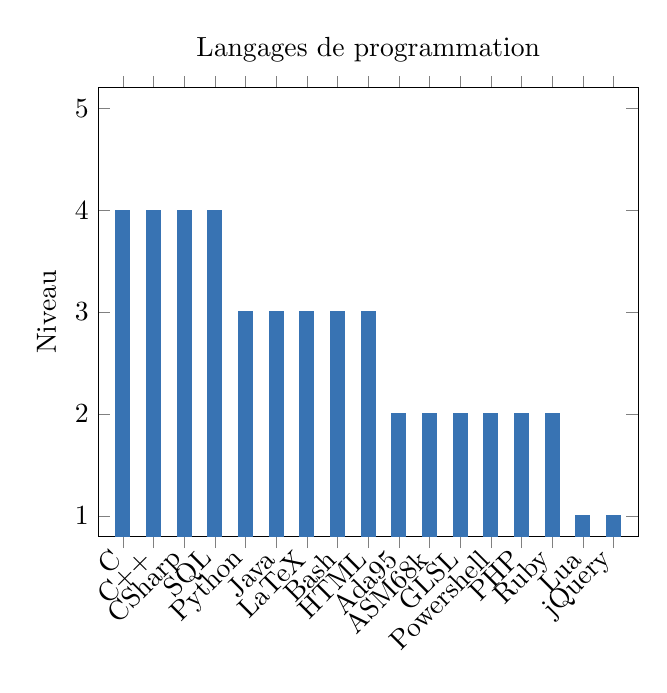
\begin{tikzpicture}
	\begin{axis}[ybar,
			title={Langages de programmation},
			enlargelimits=0.05,
			legend style={at={(0.5,-0.2)}, anchor=North, legend columns=-1},
			ylabel={Niveau},
			symbolic x coords={ C, C++, CSharp, SQL, Python, Java, LaTeX, Bash, HTML, Ada95, ASM68k, GLSL,Powershell, PHP, Ruby, Lua, jQuery},
			xtick=data,
			x tick label style={rotate=45,anchor=east},
			bar width = 5pt,
			ymax=5]
		\addplot [fill=s1,draw=s1] coordinates {(CSharp, 4)(C++, 4)(C, 4)(SQL, 4)(Python, 3)(LaTeX, 3)(HTML, 3)(Bash, 3)(Java, 3)(Ada95, 2)(ASM68k, 2)(PHP, 2)(Ruby, 2)(Powershell, 2)(Lua, 1)(jQuery, 1)(GLSL,2)};
	\end{axis}
\end{tikzpicture}

\pgfplotsset{height=3cm,width=12cm,compat=1.8}
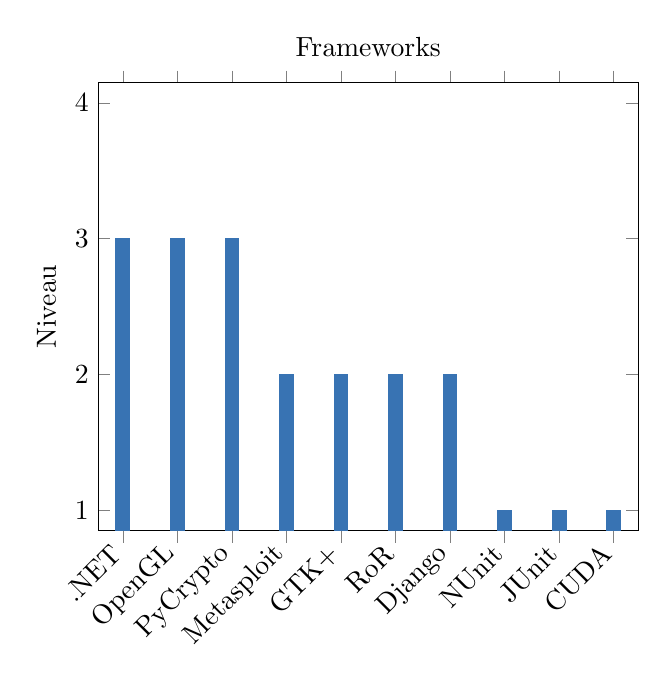
\begin{tikzpicture}
	\begin{axis}[ybar,
			title={Frameworks},
			enlargelimits=0.05,
			legend style={at={(0.5,-0.2)}, anchor=North, legend columns=-1},
			ylabel={Niveau},
			symbolic x coords={.NET, OpenGL, PyCrypto, Metasploit, GTK+, RoR, Django, NUnit, JUnit, CUDA},
			xtick=data,
			x tick label style={rotate=45,anchor=east},
			bar width = 5pt,
			ymax=4]
		\addplot [fill=s1,draw=s1] coordinates {(.NET,3)(Metasploit,2)(OpenGL,3)(GTK+,2)(PyCrypto,3)(RoR,2)(Django,2)(NUnit,1)(JUnit,1)(CUDA,1)};
	\end{axis}
\end{tikzpicture}

\cvitem{\textbf{Divers :}}{Windows, Linux, Unreal Engine 3, Unity, Méthodes de QA, UML, Merise, Git, SVN, $\mu$-controlleurs PIC et Arduino}

%----------------------------------------------------------------------------------------
%	LANGUAGES SECTION
%----------------------------------------------------------------------------------------
\vspace{6mm}

\section{Langues}
\cvitemwithcomment{Francais}{Langue natale}{}
\cvitemwithcomment{Anglais}{Avancé}{Grâce a de nombreux voyages linguistiques (Irlande, Royaume-Uni, États-Unis, Canada...)}
\cvitemwithcomment{Allemand}{Basique}{2 ans d'étude au lycée}

%----------------------------------------------------------------------------------------
%	WORK EXPERIENCE SECTION
%----------------------------------------------------------------------------------------
\clearpage
\section{Expériences}

\subsection{Vocation}

\cventry{Mai-Juin 2012}{Stage de fin de DUT}{\textsc{Groupe Folder}}{Voiron}{}{Débogage et mise à jour d'un site intranet de support aux clients de l'entreprise à l'aide du framework .NET.}

\vspace{1mm}

\cventry{Novembre 2012}{Hackfest}{}{Québec}{}{Participation aux conférences en tant qu'auditeur et participations à la cyberwar en tant que mercenaire : http://www.hackfest.ca/en/hacking-games/friday}

\vspace{2mm}

%------------------------------------------------
\subsection{Autres}

\cventry{Été 2010}{Charpentier-Couvreur}{CMI Jannon}{}{}{}
\cventry{Été 2011}{Relève des compteurs}{ERDF}{}{}{}
\cventry{Été 2013}{Tri du courrier à la pic de l'Isère}{La Poste}{}{}{}
\vspace{2mm}
%------------------------------------------------

\subsection{Projets Scolaires}
\cvlistitem{Développement d'un interpréteur Ada $\Rightarrow$ C++ en C++.}
\cvlistitem{Développement d'un logiciel de gestion de BDD, en \textbf{Java}.}
\cvlistitem{Développement de deux jeux vidéo avec \textbf{Unreal Engine 3}.}
\cvlistitem{Rédaction d'un game design document pour un RTS sur tablette nommé "The Art of War"}
\cvlistitem{Développement d'un logiciel de commandes vocales pour Windows. (Siri-like)}
\cvlistitem{Création d'une éponge de Menger en \textbf{OpenGL}}
\cvlistitem{Programmation de shaders en \textbf{GLSL}}
\cvlistitem{Implémentation d'un système de physique "masse-ressort" en C++ avec OpenGL}
\cvlistitem{Recherches académiques sur la technique de datamining utilisant les \textbf{SVM} (support vector machines)}
\vspace{2mm}

\subsection{Projets Personnels}
\cvlistitem{Développement d'outils : Eve Online mining tool; WoW addons; Rainmeter...}
\cvlistitem{Participation à http://projetmmo.bbgraph.com/ : Creation d'une BDD Postgres.}




%----------------------------------------------------------------------------------------
%	INTERESTS SECTION
%----------------------------------------------------------------------------------------
\vspace{6mm}
\section{Intérêts}

\renewcommand{\listitemsymbol}{-~} % Changes the symbol used for lists

\cvlistdoubleitem{Sports de montagne : Parapente}{Voilier}
\cvlistdoubleitem{Voyages}{Sciences et technologies}
\cvlistdoubleitem{Artisanat : Forge, Menuiserie, Bricolages divers}{Sécurité de l'entreprise}
\cvlistdoubleitem{Arts martiaux}{Jeux vidéos}
%----------------------------------------------------------------------------------------

\end{document}